The application is the database entry point, and it is projected to be run either by a government employee, a location manager or a generic user. The starting page shows the ways to access it.
\begin{figure}[h]
    \centering
    \begin{minipage}{0.75\textwidth}
        \centering
        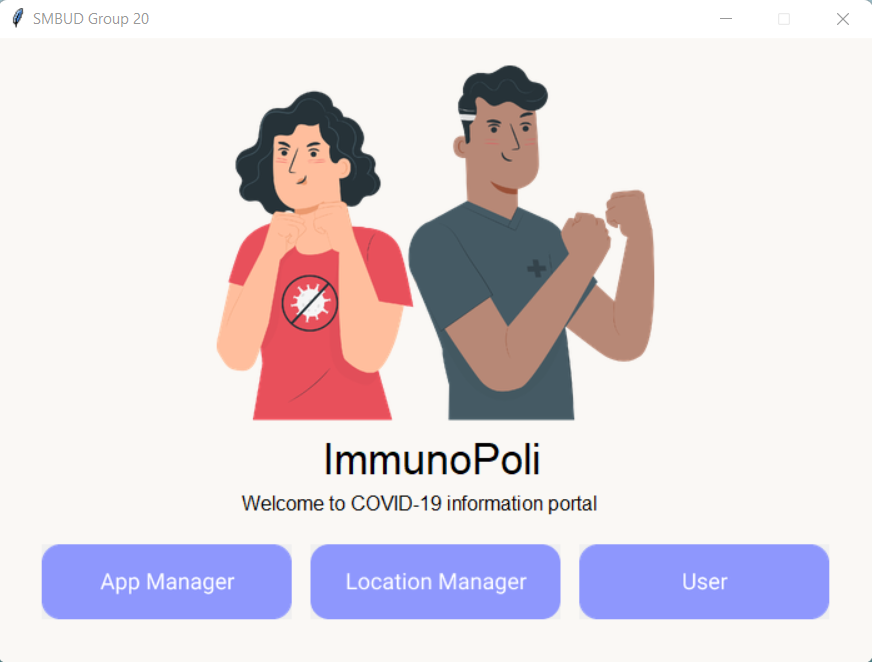
\includegraphics[width=\textwidth]{images/starting_page.png} 
        \caption{\textit{starting page}}
        \label{figure 2}
    \end{minipage}\hfill
    \begin{minipage}{0.75\textwidth}
        \centering
        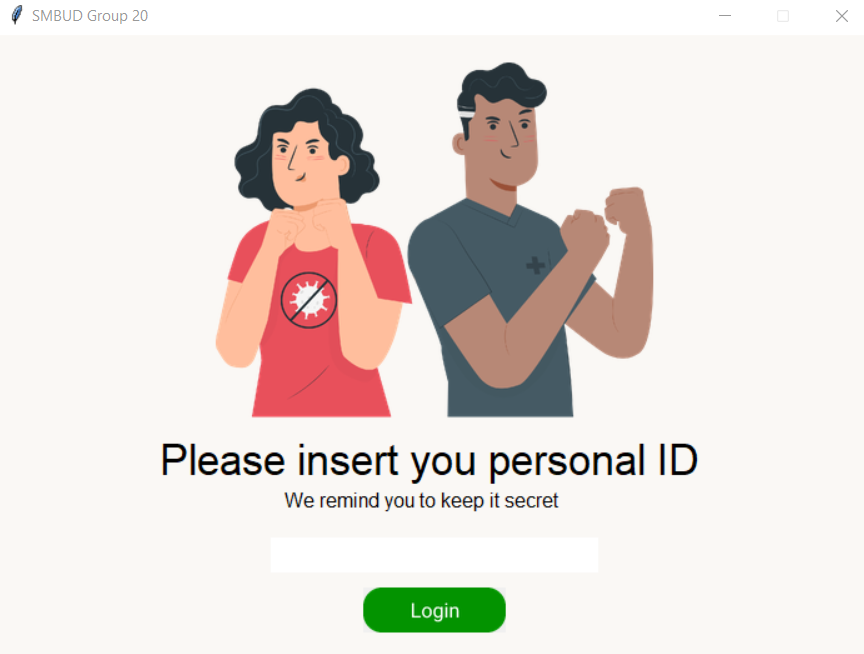
\includegraphics[width=\textwidth]{images/login_page.png} 
        \caption{\textit{login page}}
        \label{figure 3}
    \end{minipage}
\end{figure}

\newpage
\noindent
The \textbf{app manager} option is designed for an employee whose task may consist in:
\begin{itemize}
    \item adding information concerning COVID tests;
    \item monitoring COVID trends\footnote{The trends that are shown are drawn from a random database. By running them now, it may end up with different results};
    \item performing useful database queries.
\end{itemize}
\begin{figure}[h]
    \begin{subfigure}{.5\textwidth}
        \centering
        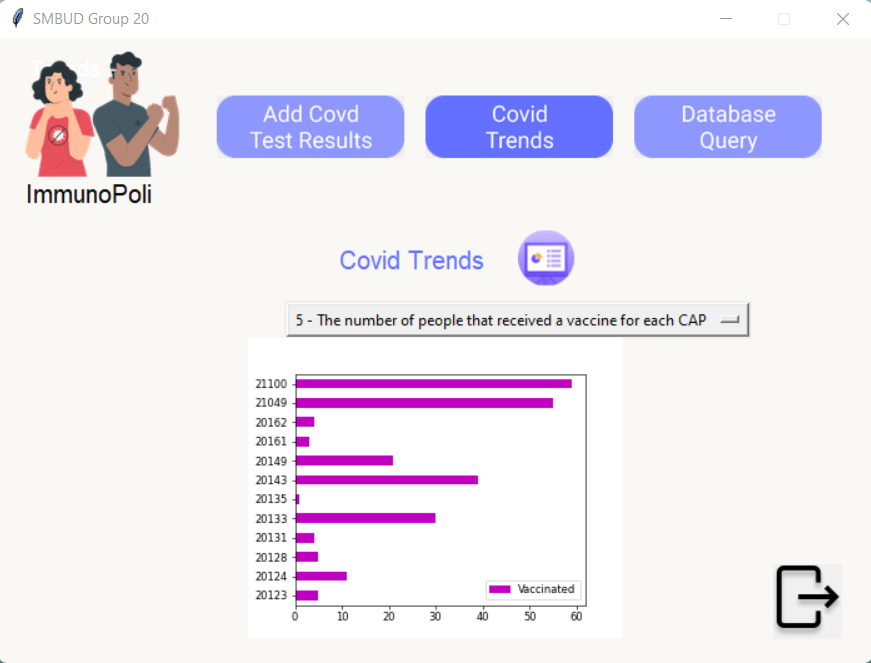
\includegraphics[width=\linewidth]{images/application_screenshots/vaccinated_per_CAP.png}  
  \caption{\textit{Number of vaccinated people organized by CAP.}}
  \label{fig: mean_age}
\end{subfigure}
\begin{subfigure}{.5\textwidth}
  \centering
  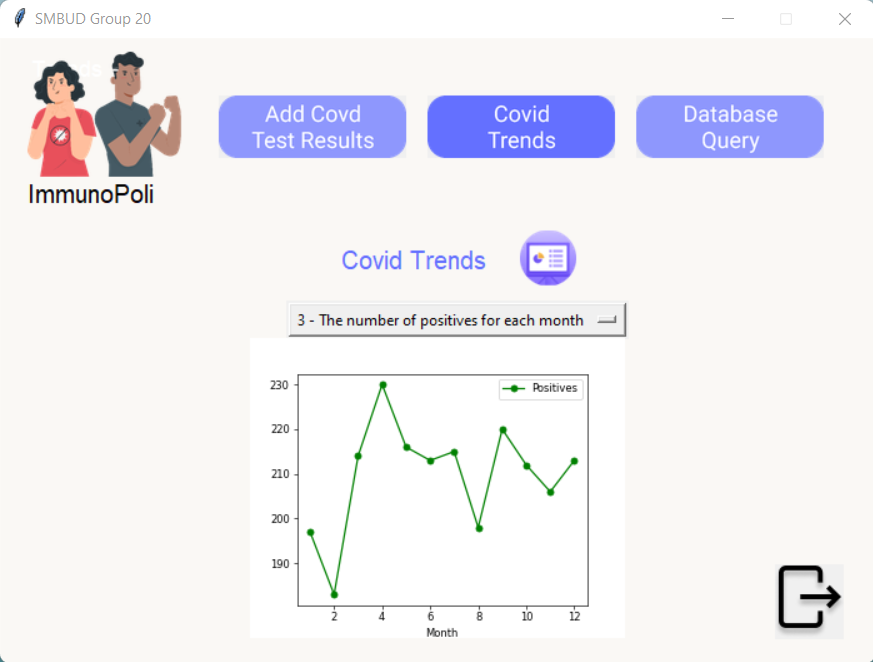
\includegraphics[width=\linewidth]{images/application_screenshots/positive per month.png}  
  \caption{\textit{Positive people trend over a twelve month horizon.}}
  \label{fig:positive_trend}
\end{subfigure}
\begin{subfigure}{.5\textwidth}
  \centering
  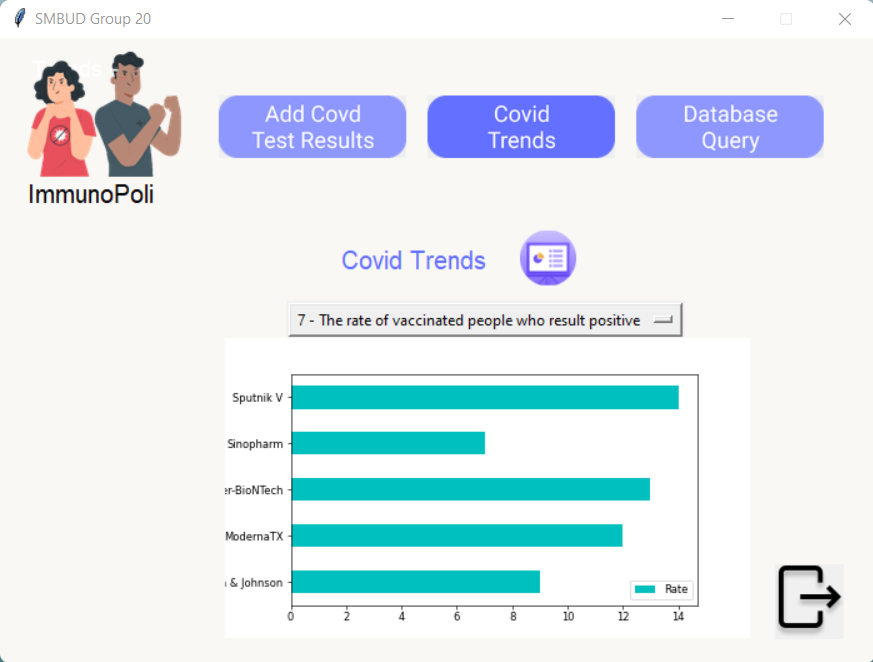
\includegraphics[width=\linewidth]{images/application_screenshots/rate_positive_vaccinated.png}  
  \caption{\textit{Percentage of positive people after at least one vaccination grouped by vaccine.}}
  \label{fig:positive_vaccinated}
\end{subfigure}
\begin{subfigure}{.5\textwidth}
  \centering
  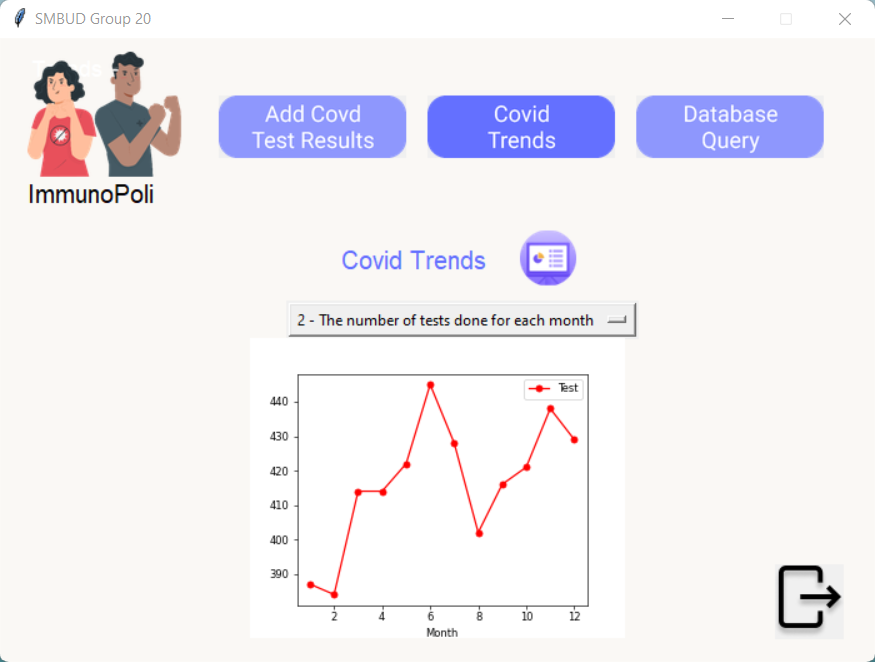
\includegraphics[width=\linewidth]{images/application_screenshots/test_trends.png}  
  \caption{\textit{Number of test performed each month.}}
  \label{fig:test_trends}
\end{subfigure}
\caption{\textit{some of the analysis that a government employee can perform from his interface.}}
\label{fig:trends}
\end{figure}
\newpage
\noindent
The \textbf{location manager} can register the people entrance inside a place. The access is granted by inserting the location ID.

\begin{figure}[h]
    \centering
    \begin{minipage}{0.485\textwidth}
        \centering
        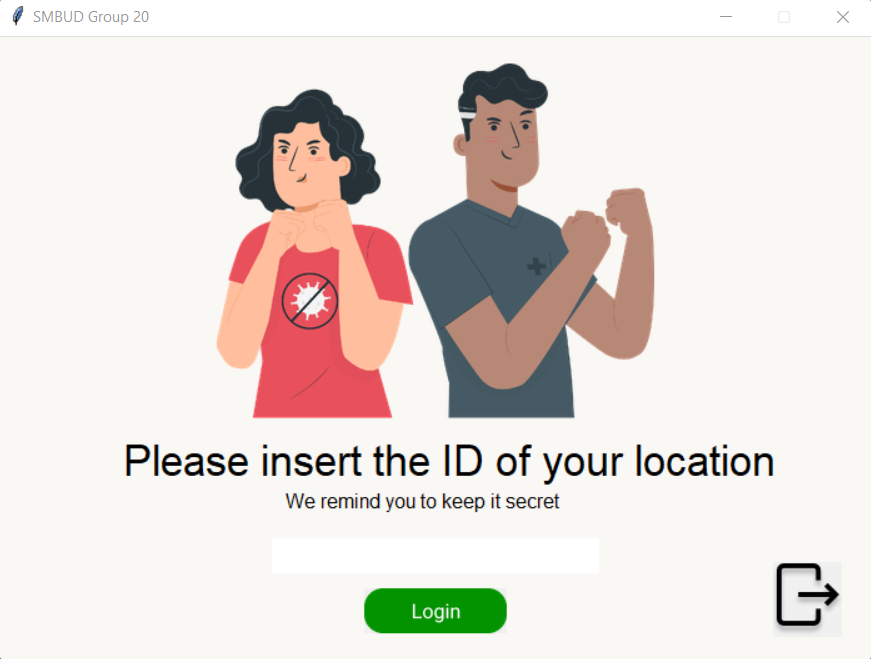
\includegraphics[width=\textwidth]{images/application_screenshots/location_manager_login.png} 
        \caption{\textit{login instruction for location managers.}}
    \end{minipage}\hfill
    \begin{minipage}{0.485\textwidth}
        \centering
        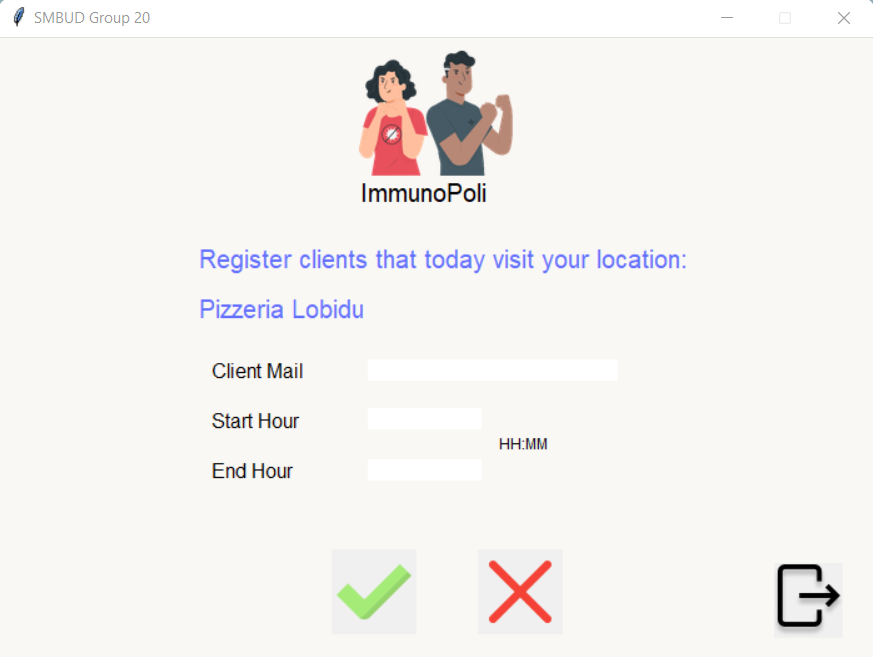
\includegraphics[width=\textwidth]{images/application_screenshots/register_visit.png} 
        \caption{\textit{dashboard for a location manager.}}
    \end{minipage}
\end{figure}



\noindent
The \textbf{generic user} has access to features that enable:
\begin{itemize}
    \item changing his/her personal information;
    \item examining the places that he has visited and the risk\footnote{The risk factor is the ratio between the number of tested positive people within ten days from the user's visit and the number of visitors in the last month.} linked to them;
    \item checking his covid exposures;
    \item seeing the history of his tests and related outcomes.
\end{itemize}

\begin{figure}[h]
    \begin{subfigure}{.5\textwidth}
        \centering
        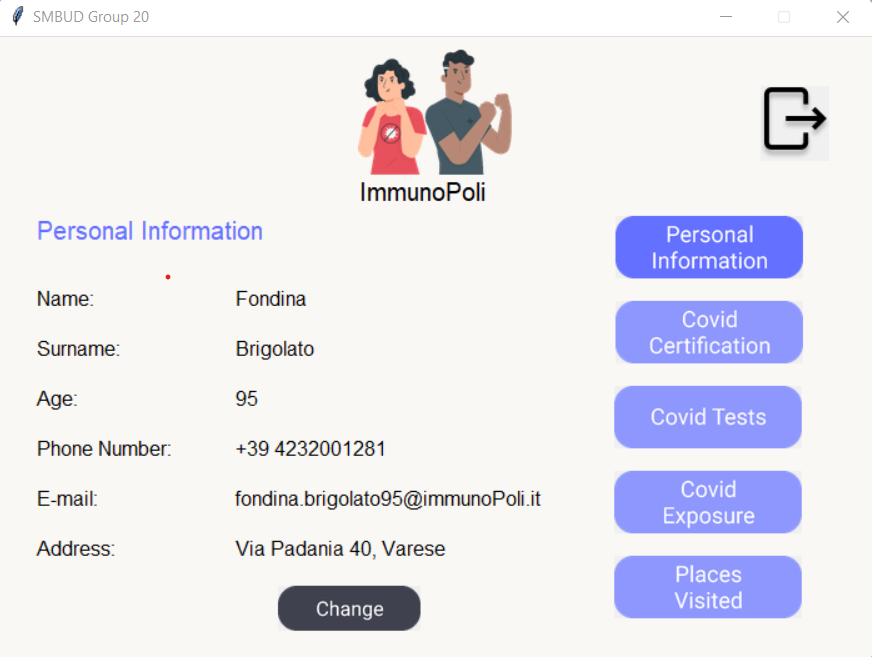
\includegraphics[width=\linewidth]{images/application_screenshots/user_information_page.png}  
  \caption{\textit{Example of the personal information stored.}}
  \label{fig: personal_information}
\end{subfigure}
\begin{subfigure}{.5\textwidth}
  \centering
  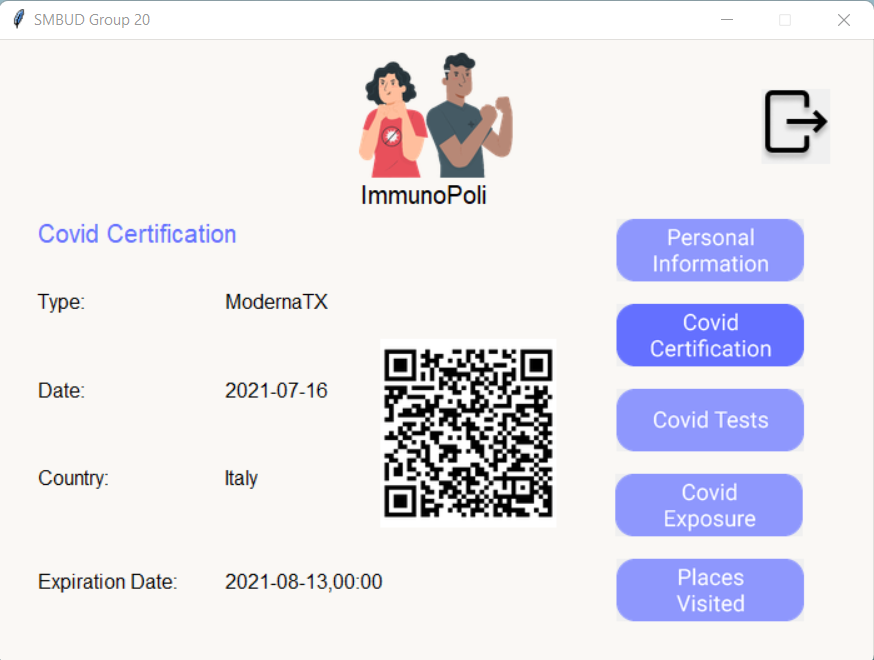
\includegraphics[width=\linewidth]{images/application_screenshots/covid_certification.png}  
  \caption{\textit{Example of covid certification lasting four weeks.}}
  \label{fig:covid_certification}
\end{subfigure}
\caption{\textit{examples of a dashboard for a generic user.}}
\end{figure}
